\chapter{Appendix}
\section{Submission File Structure}
\todo{Write section}

\section{Running the Code}
Install rustup: \\
\texttt{curl https://sh.rustup.rs -sSf | sh} \\

Install rustc 1.25.0-nightly (0c6091fbd 2018-02-04) compiler: \\
\texttt{rustup install nightly-2018-03-05} \\
\texttt{rustup default nightly-2018-03-05} \\

Verify the version is correct using: \\
\texttt{rustc --version} \\

Create a new crate and write sequential code: \\
\texttt{cargo init} \\

Under \texttt{[dependencies]} in \texttt{Cargo.toml}, add: \\
\texttt{auto\_parallelise = \{ version = "0.1.0", git = "https://github.com/MichaelOultram/FYP/", branch = "release" \}} \\

At the top of your \texttt{lib.rs} or \texttt{main.rs} file, add: \\
\texttt{\#![feature(plugin)]} \\
\texttt{\#![plugin(auto\_parallelise)]} \\

At the top of every function, add: \\
\texttt{\#[autoparallelise]} \\

Compile the code twice using (the first time will fail): \\
\texttt{cargo build --release} \\

Run the parallelised code using: \\
\texttt{cargo run --release}

\section{References}
\printbibliography[heading=none]

%\section{Project Proposal and Scientific Paper}
%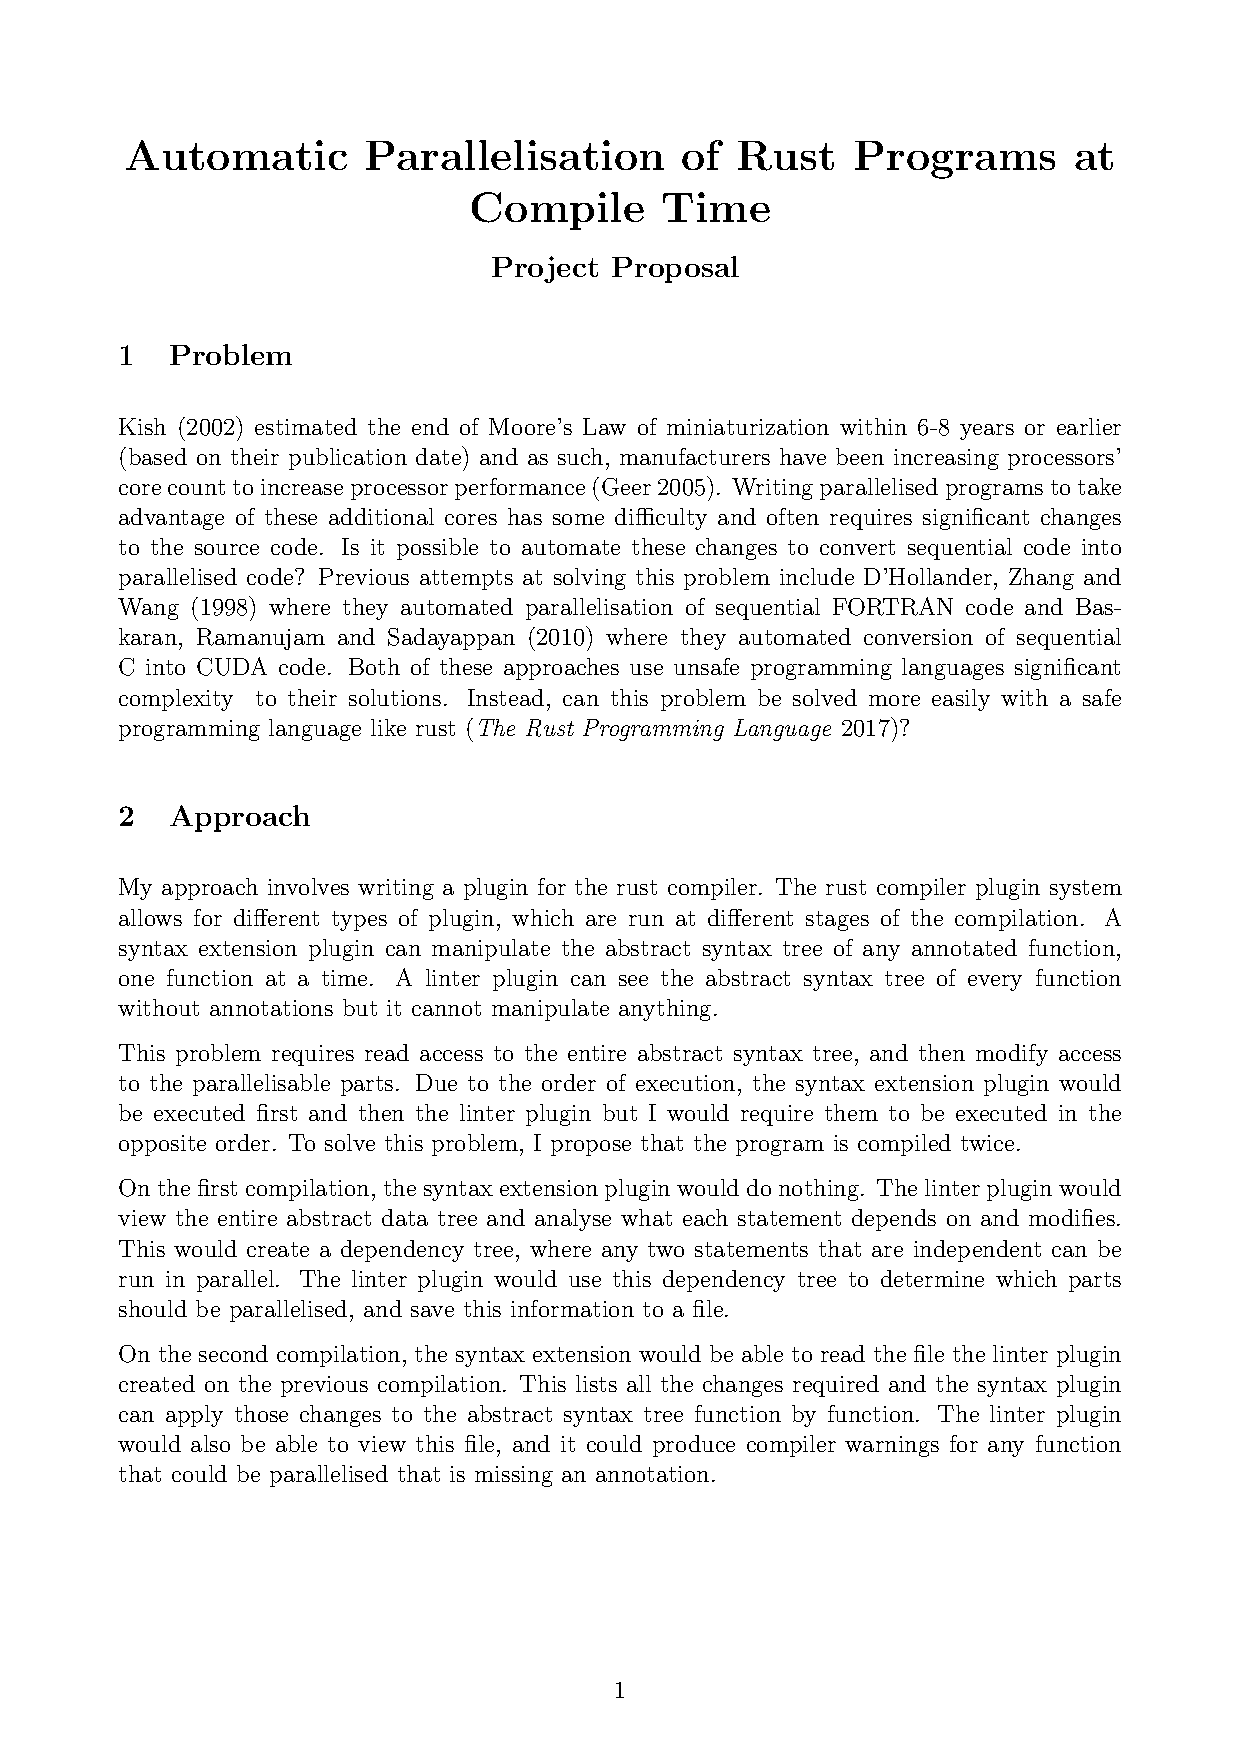
\includepdf[pages=-]{../0-Proposal/main.pdf}
%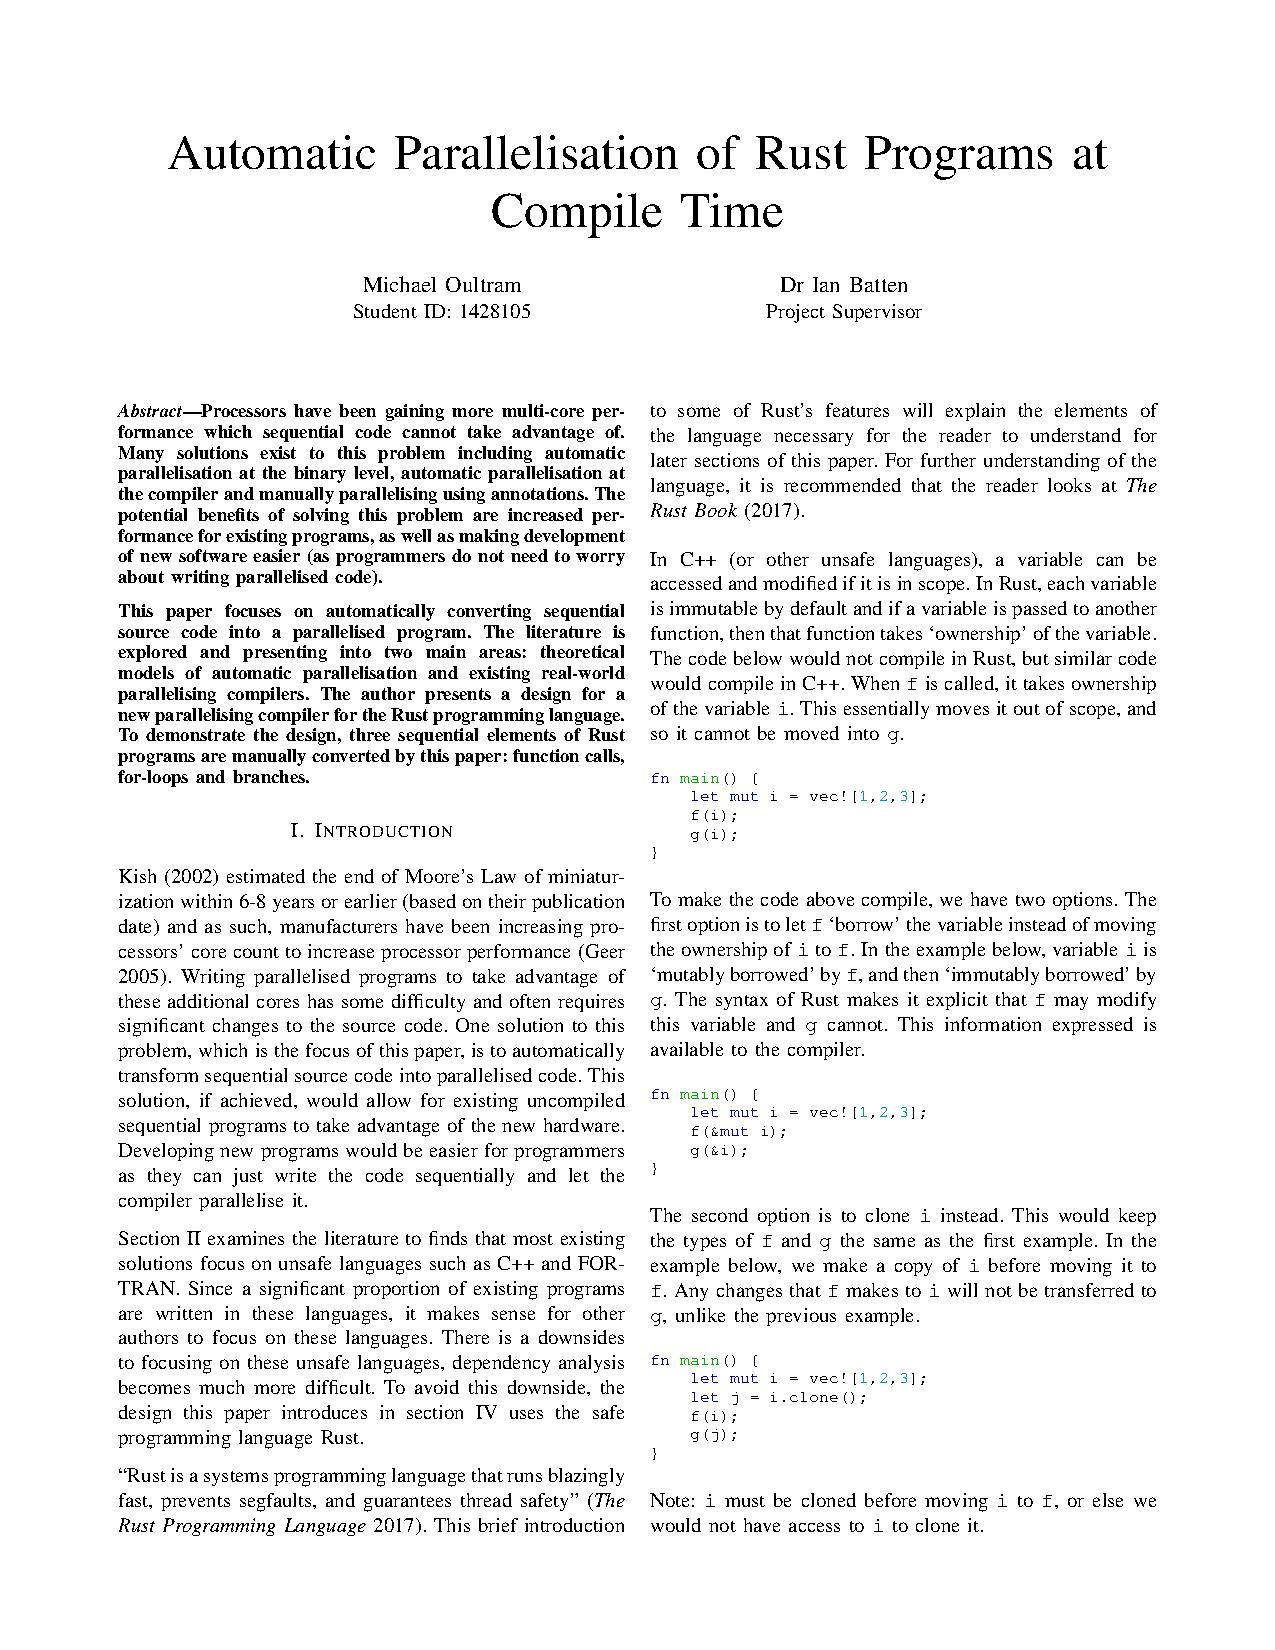
\includepdf[pages=-]{../1-Scientific-Paper//main.pdf}
